\section{Proposed extensions}\label{sec:extension}
%\matthias{Here we will list the things we miss in each language, and introduce possible ways of implementing them and ways to learn from eachother}
\matthias{How does ProB add HO, and what can we learn from them (and vice-versa)}
In this section, we compile a list of missing language constructs, and introduce possible ways of implementing them and ways to learn from eachother.
\subsection{Language}
HO is sometimes criticized as being to expressive.
Sometimes however, the additional structure HO exhibits allows solvers to perform better.
For example, in this case HO preserves the local coherence and independence of the different examples, a property that the solver could leverage to become more efficient.
\subsection{solver}

\begin{figure}
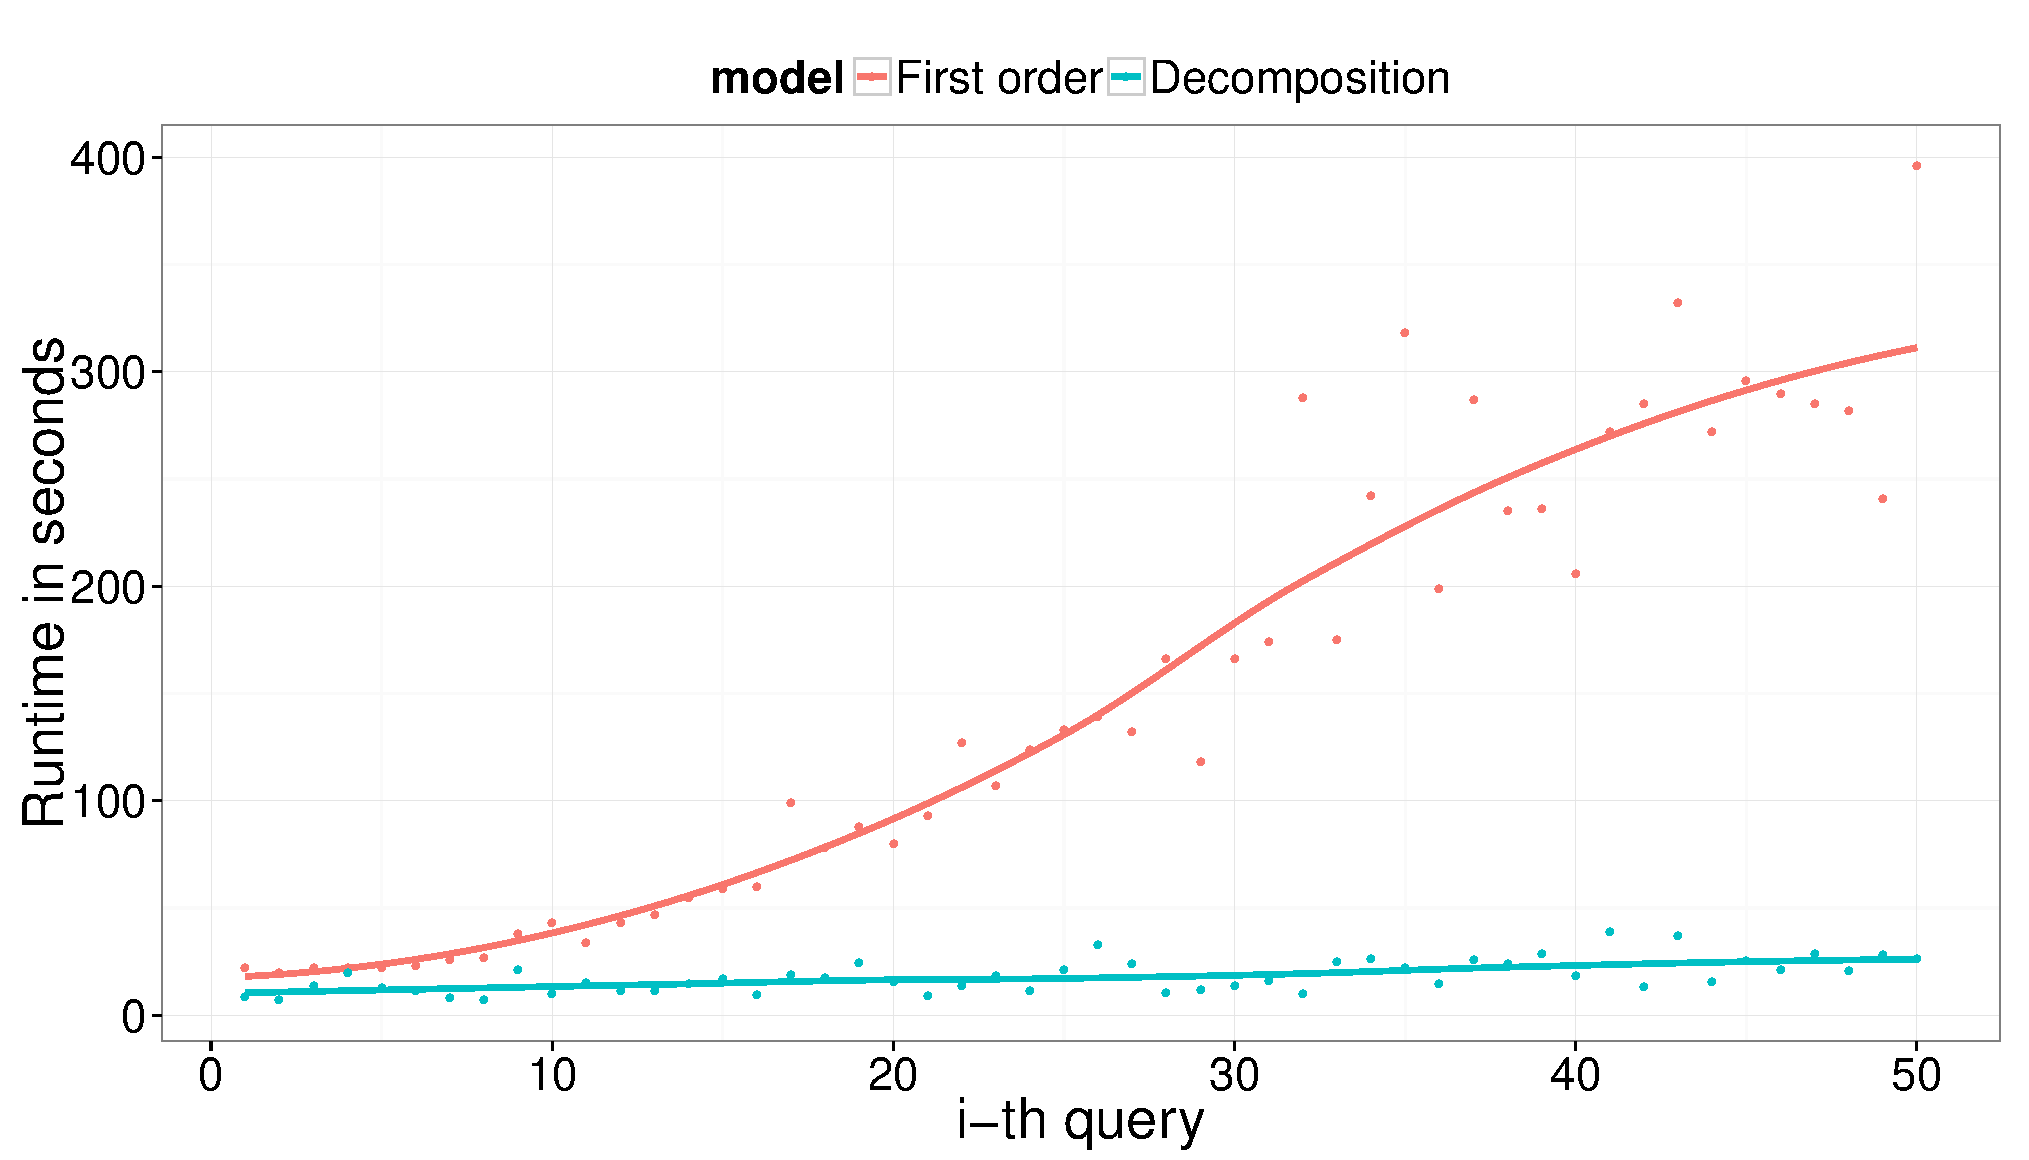
\includegraphics[width=\linewidth]{extra/figure_comparison_yoshida.pdf}
\end{figure}


\subsubsection{Oracles}
\subsubsection{Benders decomposition}

\subsection{Faithful encoding}
\matthias{In this subsection, we show a new encoding, which is not yet supported in IDP, and argue that it is more faithful to the problem with respect to the definition as given in Def~\ref{def:gm2}.}
\begin{alltt}
  homomorphism(<Edge1, Label1>, <Edge2, Label2>) \(\iff\)
      \big(\(\exists\) f: (\(\forall\) x, y : x \(\neq\) y \(\Rightarrow\) f(x) \(\neq\) f(y)) \(\wedge\)
      (\(\forall\) x, y : Edge1(x, y) \(\implies\) Edge2(f(x), f(y))) \(\wedge\)
      (\(\forall\) x : Label1(x) = Label2(f(x)))\big)

  isomorph(<Edge1, Label1>,<Edge2, Label2>) \(\iff\)
      \big(\(\exists\)f : (\(\forall\)x,y:x\(\neq\)y\(\implies\)f(x)\(\neq\)f(y)) \(\wedge\)
      (\(\forall\) x, y : Edge1(x, y) \(\iff\) Edge2(f(x), f(y))) \(\wedge\)
      (\(\forall\) x : Label1(x) = Label2(f(x)))\big).

  \textbraceleft
  reachable(x, y, <Edge, Label>) \(\leftarrow\) Edge(x, y) \(\lor\) Edge(y, x).
  reachable(x, y, <Edge, Label>) \(\leftarrow \exists\) : reachable(x, z, <Edge, Label>) \(\wedge\) reachable(z, y, <Edge, Label>).
  \textbraceright

  //\(\forall\)Pat represents quantification over a predicate Pat/2. 
  //A pattern is represented by its Edge relation. 
  \(\forall\)P : pattern(P) \(\implies\) \#\textbraceleft Pos : positive(Pos) \(\wedge\) homomorphism(P, Pos) \textbraceright \(\geq\) \(N{+}\).
  \(\forall\)P : pattern(P) \(\implies\) \#\textbraceleft Neg : negative(Neg) \(\wedge\) homomorphism(P, Neg) \textbraceright \(\leq\) \(N_\).
  \(\forall\)P : pattern(P) \(\implies\) x, y : reachable(x,y, P). 
  \(\forall\)P,P2 : pattern(P)\(\wedge\)pattern(P2)\(\wedge\)P\(\neq\)P2 \(\iff\) \(\neg\)isomorph(P, P2).

\end{alltt}

This encoding compactly specifies the graph mining problem, in a way that closely corresponds to its mathematical definition.
To allow inferences on this theory, extended solver support is necessary.
We now identify possible ways in which a solver can provide this additional support:

\subsubsection{Data representation}

One possible way to solve these higher order theories is based on the disjoint union technique: 
We automatically derive a \emph{disjoint union} specification from this higher order theory.
By analyzing the different rules in the specification, the solver can derive that the only \matthias{one of the? (zie later)} higher order objects consist of an edge relation and a labeling function.
It can then introduce these relations automatically, indexed by an identifier.
Quantifications over these higher order objects become quantifications over these identifiers.
\matthias{Furthermore the solver must also detect the existential quantification of the function $f$.
This too leads to a disjoint union }

Another way is to automatically introduce separate predicates and functions for each higher order object. 
The solver subsequently replicates the necessary rules specified for these separate predicates and functions. \matthias{Dit gaat eigenlijk alleen in combinatie met de subsolver approach, omdat ik in het geval van een universele quantificatie over een predicaat waar gezocht wordt niet weet hoeveel keer ik de regels moet instantiëren.}

\subsubsection{Negative contexts}
First, the solver must detect existential higher order quantifications.
When an existential quantification occurs in a negative context, 

\matthias{Wanneer je (lokaal) herschrijft naar ESO komen al je coNP problemen (die je zéker in een subsolver moet steken) voor in negatieve context. Ik dacht dus ook dit apart te behandelen van de data representatie. Hier moet echter de kanttekening van boven bij gemaakt worden dat alleen in dit geval de replication methode haalbaar lijkt...}